\section{3-D Punktwolke}
\label{3-D Punktwolke}
In dieser Aufgabe soll aus einer Reihe von Bildern eines Objekts, welche von verschiedenen Kamerastandpunkten aufgenommen wurden, eine 3D Punktwolke des Ob-jekts berechnet werden. 

\subsection{Algorithmus}
In diesem Kapitel wird der gesamte Algorithmus erklärt, der von der Bildserie zur 3D Punktwolke führt. Er enthält einige komplexe Unteralgorithmen die in den nächsten Kapiteln erläutert werden. Die grobe Vorgehensweise ist an [1] angelehnt.
Zunächst müssen die Bilder des Objekts geladen werden. Dabei ist es wichtig dass sie in der richtigen Reihenfolge geladen werden, da aufeinanderfolgende Bilder eine Überlappung von mindestens 50\% haben müssen. Außerdem müssen die Bilder in Grauwertbilder umgewandelt werden, da die darauffolgenden Algorithmen nur mit 1-kanaligen Bildern umgehen können. Zusätzlich müssen die Kameraparameter der Kamera, mit denen die Bilder aufgenommen wurden, geladen werden. Die Ermittlung der Kameraparameter wird in Kapitel XX.XX  beschrieben.
Nun wird das erste Bild verarbeitet, indem es über die Funktion undistortImage und die Kameraparameter verzeichungsfrei (s. Kapitel XX.XX) gemacht wird.
Als nächstes werden auf dem ersten Bild markante Punkte über den Harris Corner Detector (s. Kapitel Korrespondenzanalyse) ermittelt. Nun wird der erste Kamerastandpunkt, er ist der Referenzstandpunkt im Nullpunkt mit der Einheitsmatrix als Orientierung, mitsamt der markanten Punkte in eine Datenstruktur mit dem Namen ViewSet gespeichert. Diese speichert alle Parameter eines Kamerastandpunkts und ordnet diesen eine ID zu. Beim ersten Bild ist dies die ID 1.
Es folgt eine Schleife die über alle Bilder Iteriert. Mit dem nächsten Bild wird nun analog zum ersten Verfahren, es wird verzeichnungsfrei gerechnet und seine markanten Punkte werden ermittelt. Nun werden aber Punkte zwischen dem vorigen und dem gerade in der Schleife untersuchten Bild ermittelt die in beiden Bildern vorkommen. Solche Punkte werden als Matches bezeichnet. Die genaue Erläuterung der Berechnung von Matches folgt in Kapitel Korrespondenzanalyse.
Mit diesen ermittelten Matches kann nun eine sogenannte Fundamentalmatrix berechnet werden. Diese enthält Informationen über die intrinsischen und extrinsischen Kameraparameter. Das genaue Vorgehen zur Berechnug der Fundamentalmatrix sowie deren Eigenschaften werden in Kapitel Schätzen der Fundamentalmatrix erläutert. 
Aus der Fundamentalmatrix kann durch Multiplikation der intrinsischen Kameraparameter beider Kameras (hier identisch da gleiche Kamera) die Essentielle Matrix berechnet werden, die nur noch Informationen über die extrinsischen Kameraparameter enthält. Im nächsten Schritt kann nun aus der Essentiellen Matrix die Lage und Orientierung der Kamera ermittelt werden. (siehe Kapitel Schätzen der Kamerapose aus der Fundamentalmatrix).
Die berechnete Kamerapose sowie die Matches werden mit der nächsten ID in die ViewSet  Datenstruktur gespeichert. Da zwischen den Bildern jeweils nur relative Posen berechnet werden, müssen diese zuvor noch mit der Position und Orientierung des vorigen Standpunkts verechnet werden. 
Im letzten Schritt innerhalb der Schleife wird nun das aktuelle Bild zum vorigen Bild, sodass zwischen diesem und dem nächsten wieder eine Korrespondenzanalyse sowie die Ermittlung der Kamerapose berechnet werden kann.
Sind alle Kameraposen und deren Matches im ViewSet gespeichert kann nun eine Triangulation der Matches stattfinden. Dazu werden mit der Funktion findTracks Punkte ermittelt die in mehreren Bildern (mind. 2) auftauchen. Über diese Tracks wird eine Triangulation wie im Kapitel Triangulation beschrieben durchgeführt. Ergebnis sind Punkte im 3D Raum die zum Schluss noch geplottet werden.
Das gesamte Vorgehen wird hier nocheinmal im Pseudocode zusammengefasst.
\begin{figure}[ht]
    \centering
    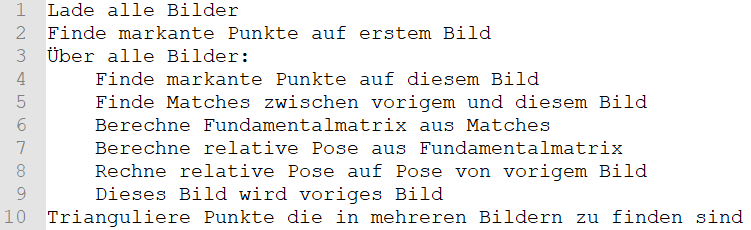
\includegraphics[scale=0.75]{Figures/Pseudocode.PNG}
    \caption{Pseudocode}
\end{figure}

\subsection{Kamerakalibrierung}
Die Kalibrierung der Kamera ist wichtig, da die Abbildung jeder Kamera ein wenig anders ist. So unterscheiden sich zum Beispiel die Brennweiten von Gerät zu Gerät geringfügig und jede Kamera hat ihre eigenen Verzeichnungsfehler.
Es gibt zwei Arten von Verzeichnungsfehlern, die tangentiale und die radiale. Die ra-diale Verzeichnung entsteht durch die Krümmung der Linse bzw. kleine unebenheiten die bei der Produktion entstanden sind. Die Tangentiale Verzeichnung entsteht dadurch dass der Fotochip nicht exakt parallel zur Linse eingebaut wurde. Die Folgenden Bild-er zeigen die Auswirkungen von tangentialer und radialer Verzeichnung.

BILDBILDBILD

Matlab bietet eine Applikation die aus Bildern von einem Kalibrierungsboard die Ka-meraparameter schätzt. Dazu muss das Board aus vielen verschiedenen Positionen (ca. 20) fotographiert werden. 

\begin{figure}[ht]
    \subfigure {
    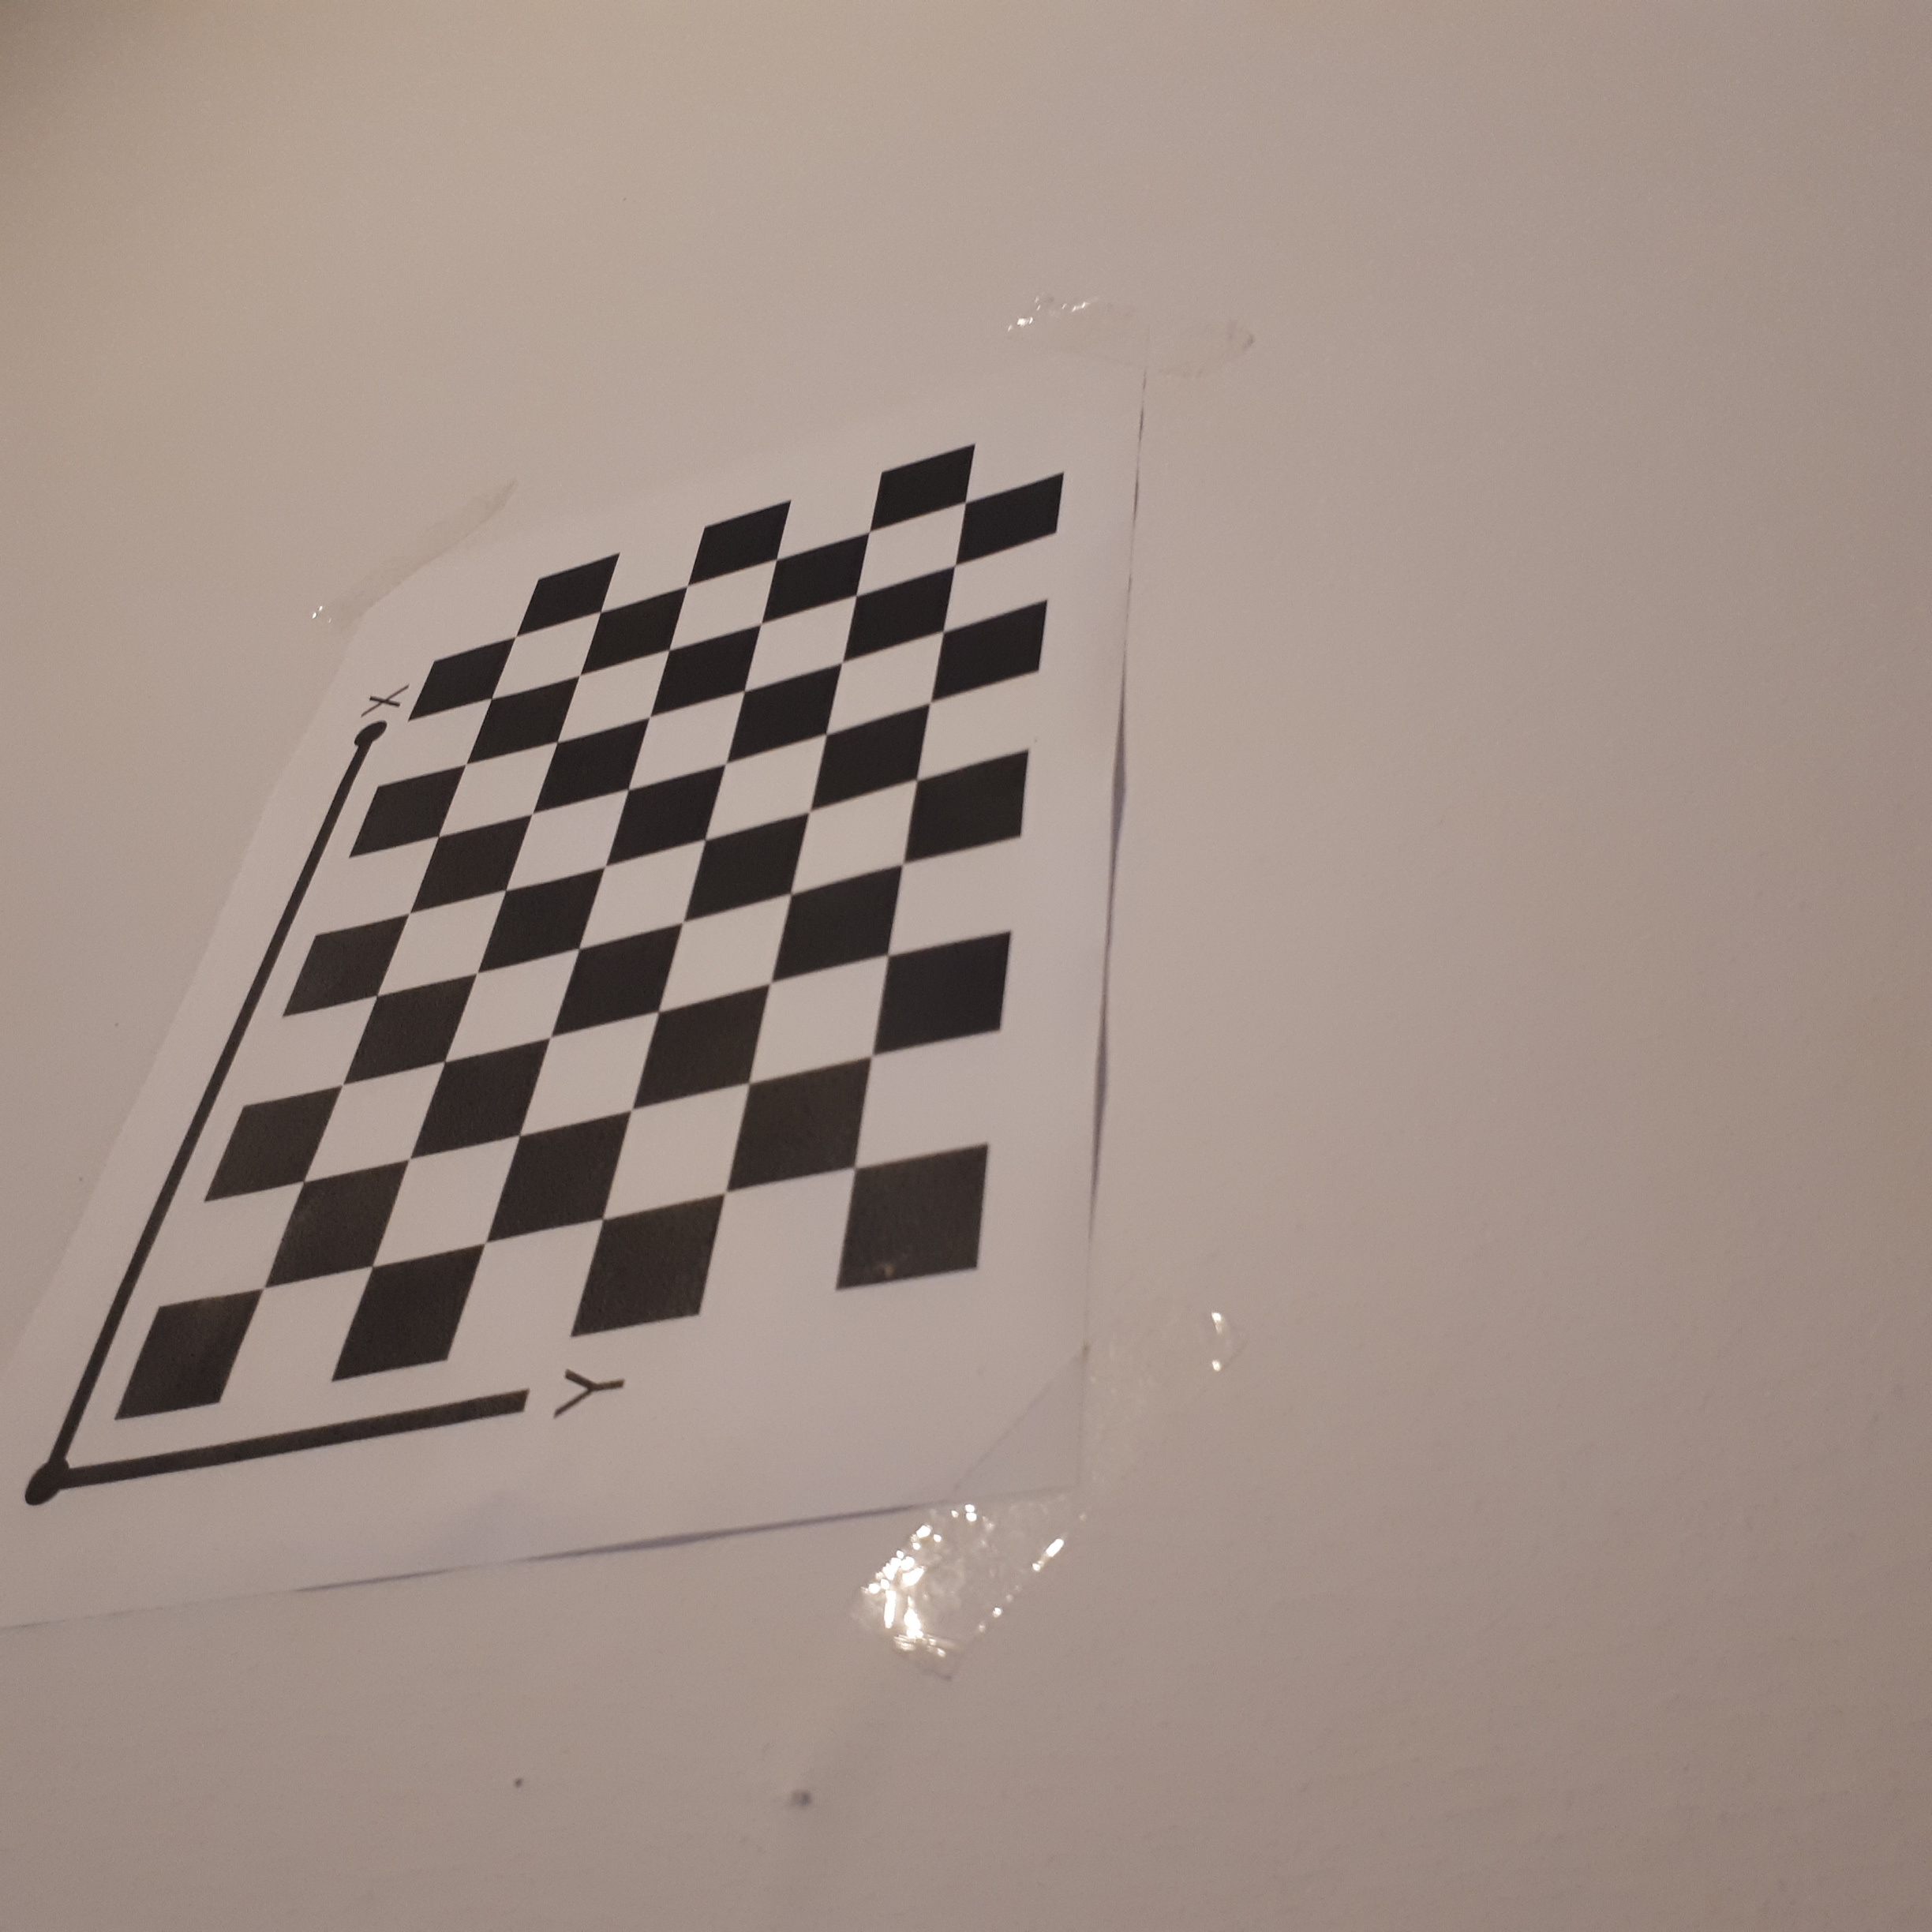
\includegraphics[scale=0.05]{Figures/Kalib1 (1).jpg}
    }
    \subfigure{
    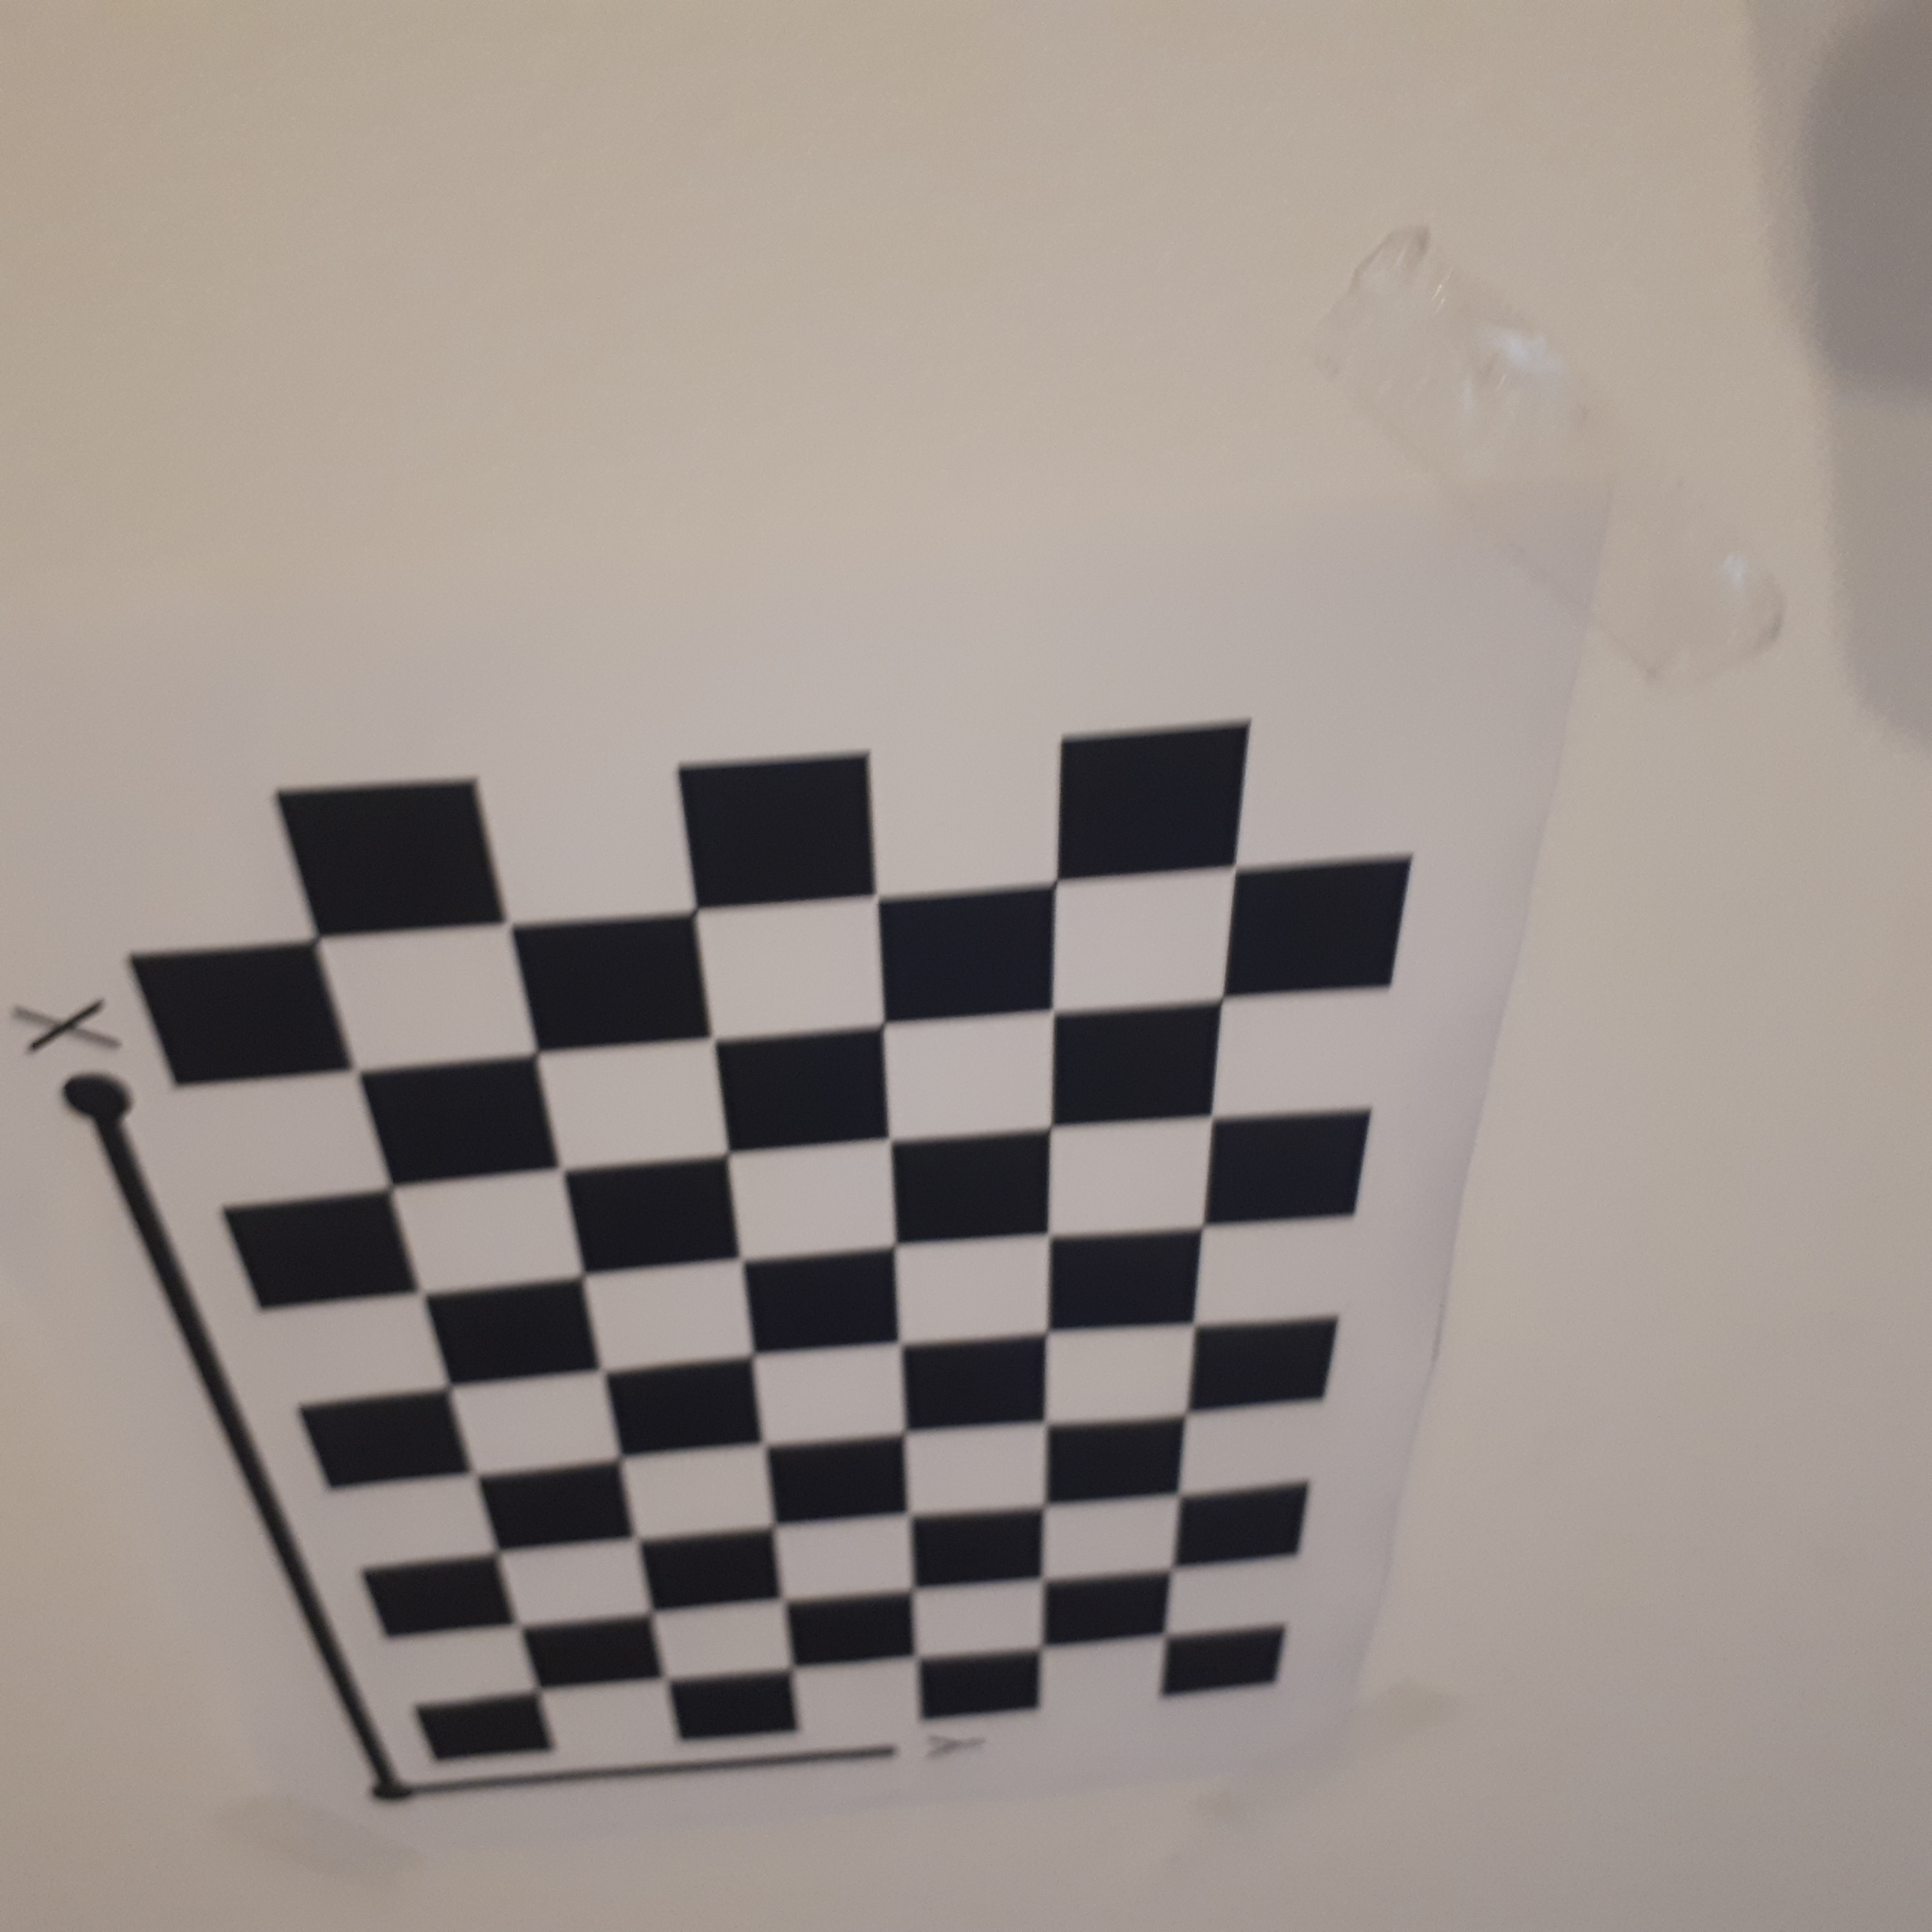
\includegraphics[scale=0.05]{Figures/Kalib1 (2).jpg}
    }
    \subfigure{
    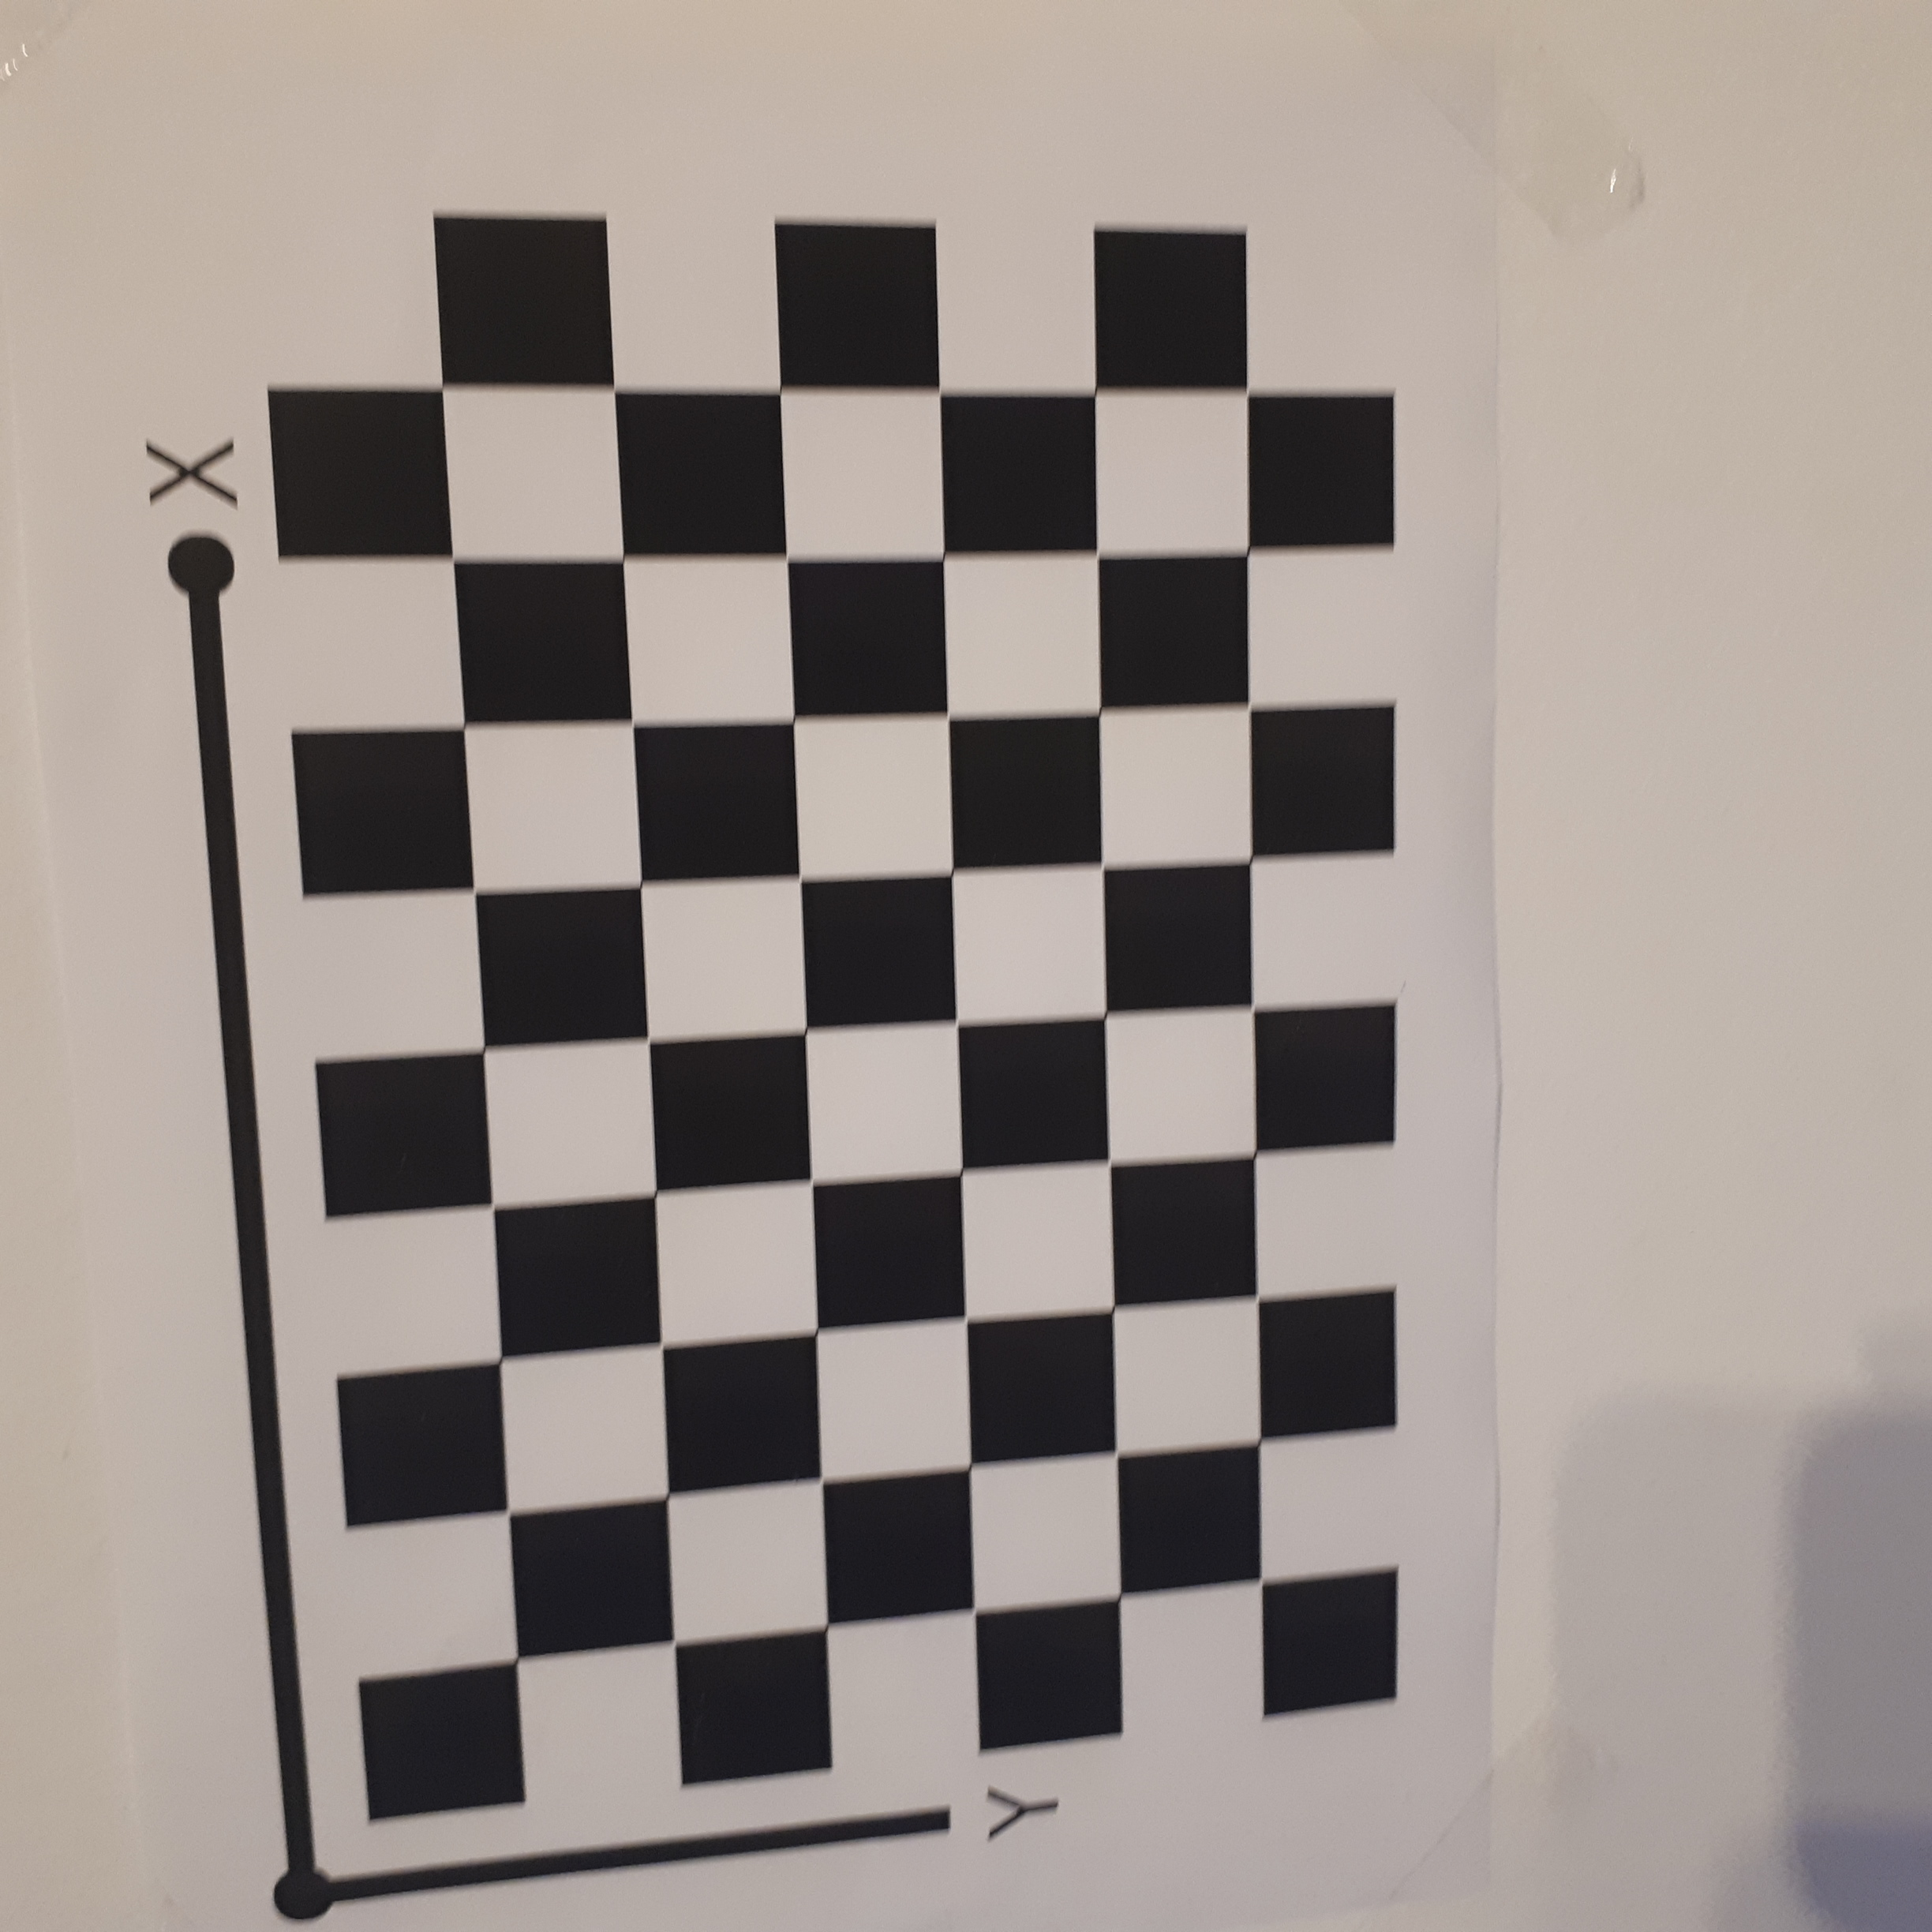
\includegraphics[scale=0.05]{Figures/Kalib1 (3).jpg}
    }
    \subfigure{
    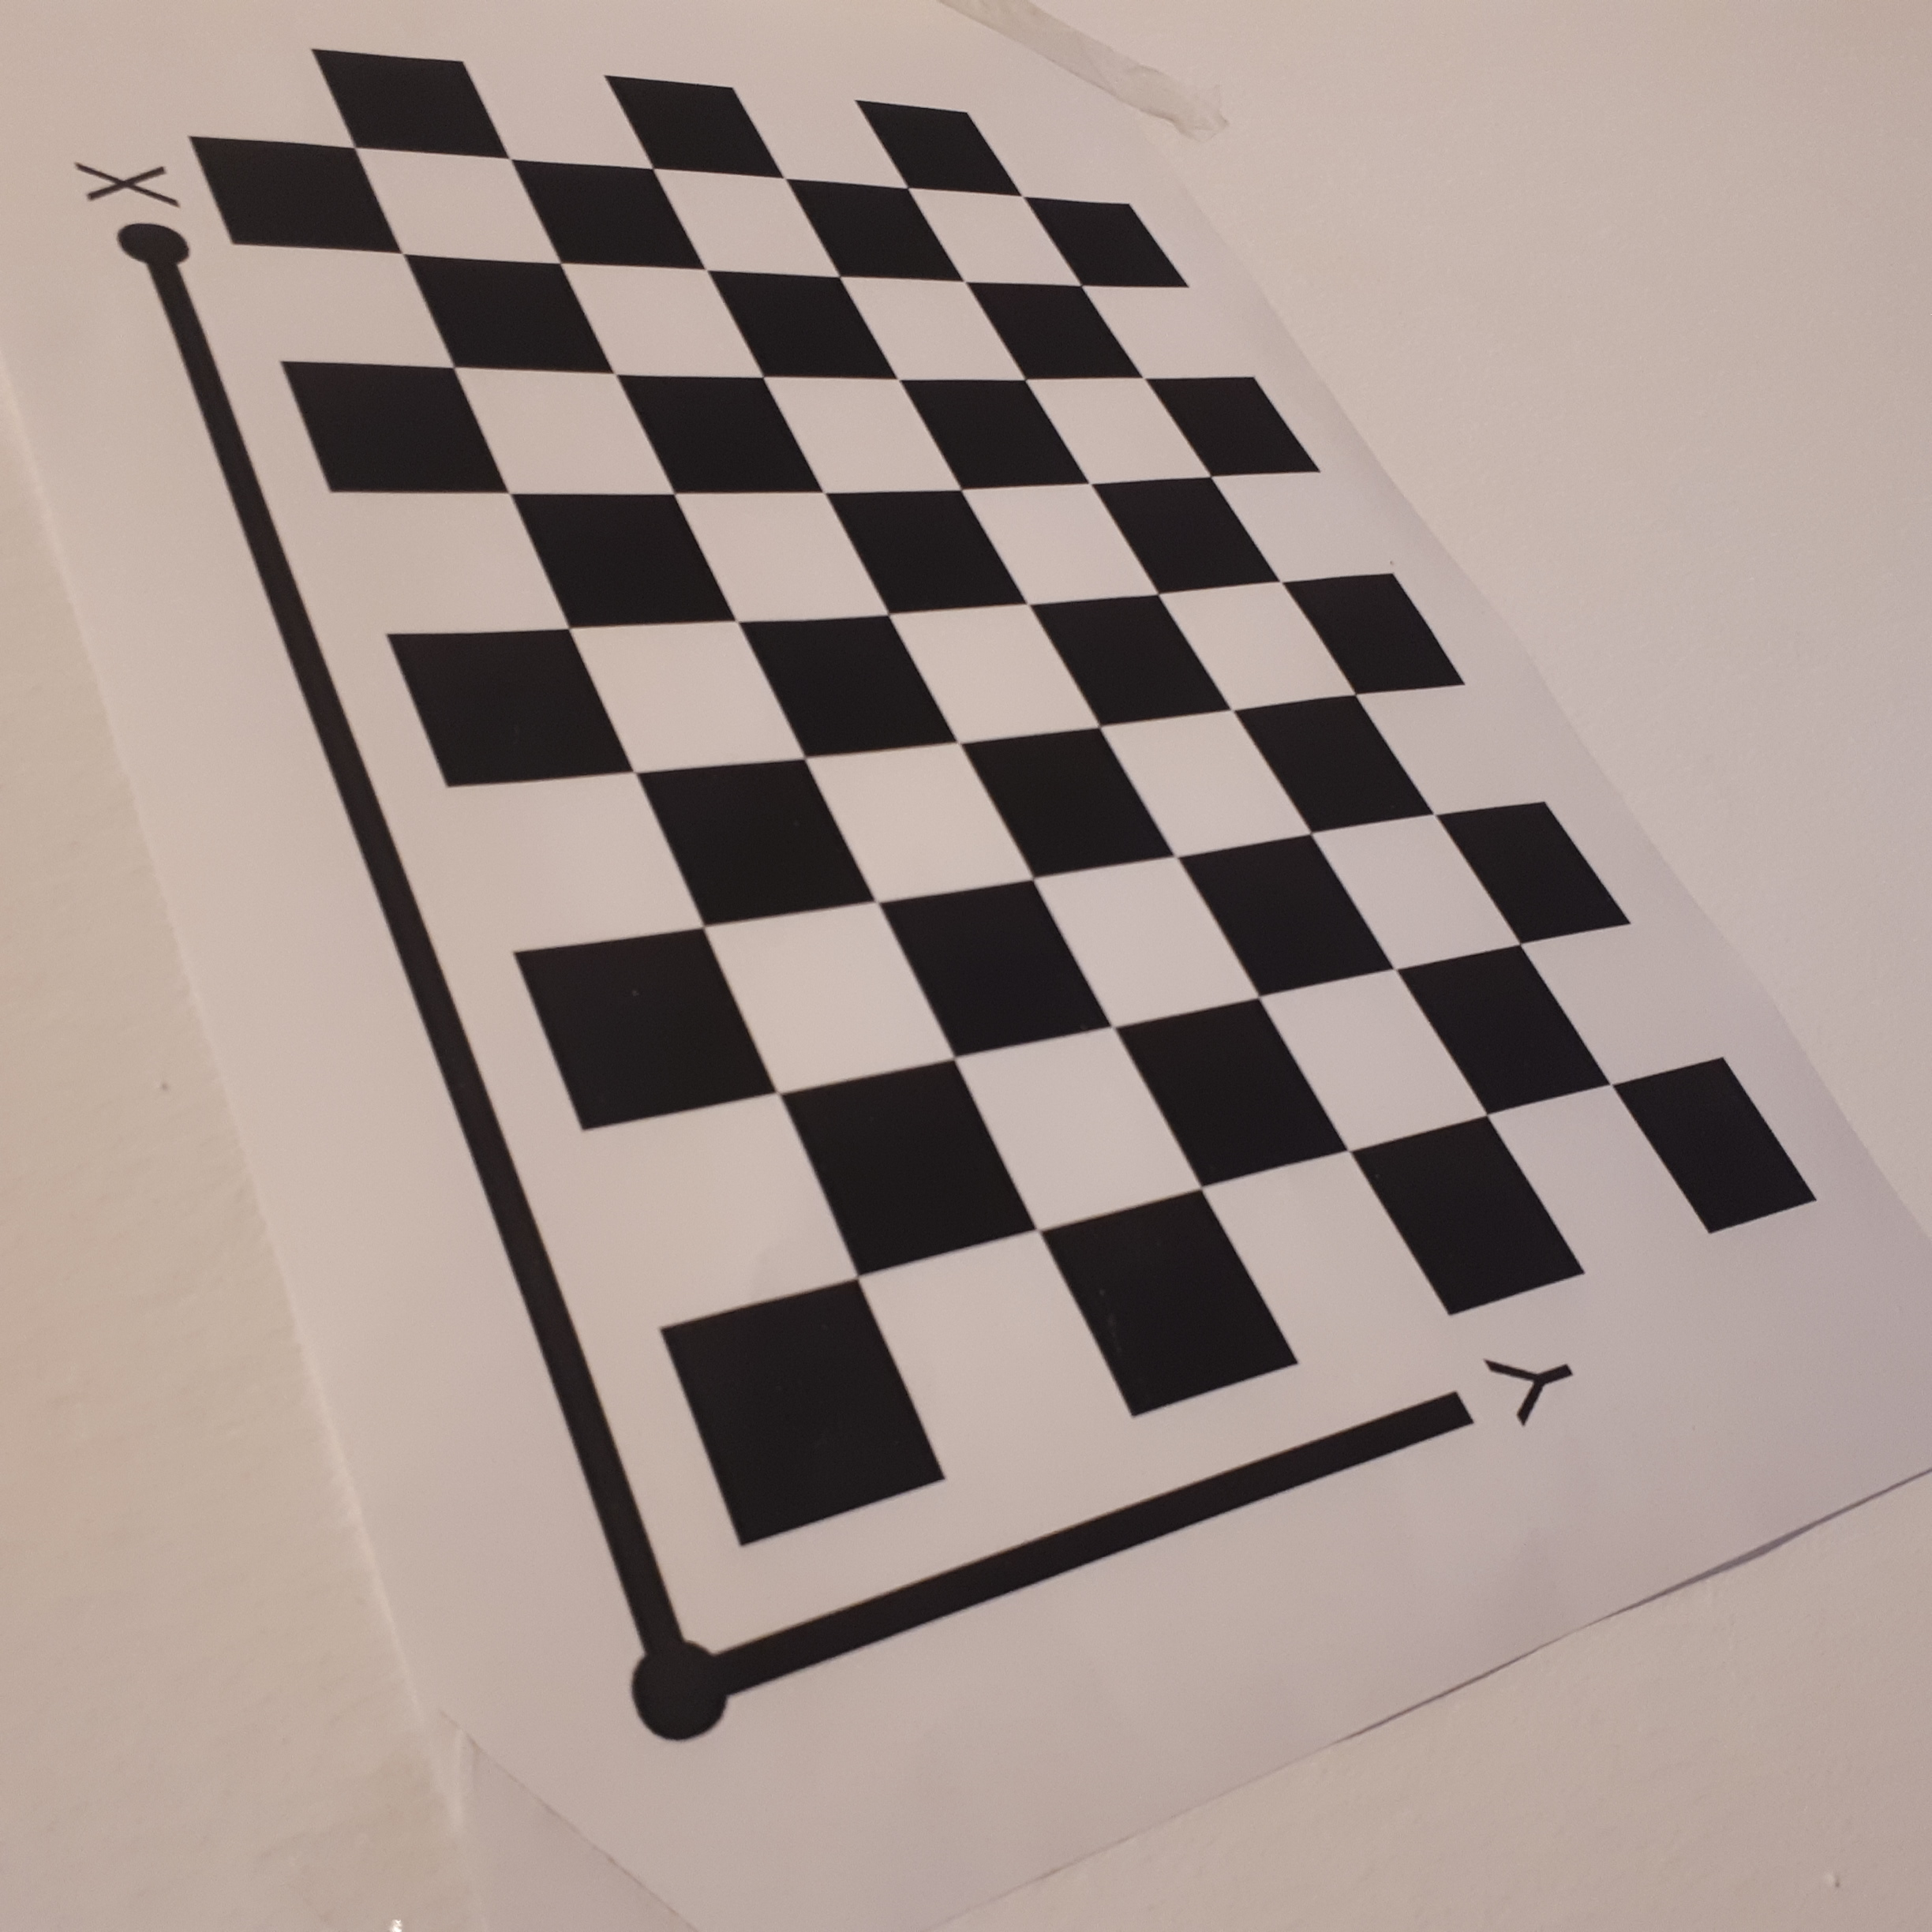
\includegraphics[scale=0.05]{Figures/Kalib1 (4).jpg}
    }
    \caption{Bilder des Kalibrierungsboards}
\end{figure}

Aus diesen Bildern und der Information wie groß die Abstände der einzelnen Quadrate sind ermittelt die Applikation extrinsische und intrinsische Kameraparameter. Diese können als CameraParameters Objekt gespeichert und an anderer Stelle wieder geladen werden. Das CameraParamters enthält viele Informationen über die Kamera und die Kalibrierung. Von besonderer Bedeutung für diesen Einsatzweck sind hier die Einträge RadialDistortion und TangentialDistortion, welche für das Entzerren des Bildes wichtig sind. Außerdem wird die IntrinsicMatrix benötigt um aus der Fundamentalma-trix die Essentielle Matrix zu berechnen. 

\subsection{Korrespondenzanalyse}

\subsection{Schätzen der Fundamentalmatrix}
Die Fundamentalmatrix ist eine Matrix, welche die Geometrie zweier Kameras zue-inander sowie deren intrinsische Parameter beschreibt. Sie stellt die algebraische Repräsentation der Epipolargeometrie dar.

\subparagraph{Epipolargeometrie}
Die Epipolargeometrie liefert eine geometrische Beschreibung für zwei Ka-meraperspektiven auf einen Punkt in der Realität. Der Vorteil dieses Modells im Gegensatz zu anderen Modellen wie der Standardstereogeometrie ist, dass die Kameras eine beliebige Brennweite haben können und sie nicht in einer Ebene liegen müssen. Dieses Modell past also gut zur gestellten Aufgabe, da das Objekt von vielen unter-schiedlichen frei positionierten Kamerastandpunkten aufgenommen wird.
\begin{figure}[ht]
    \centering
    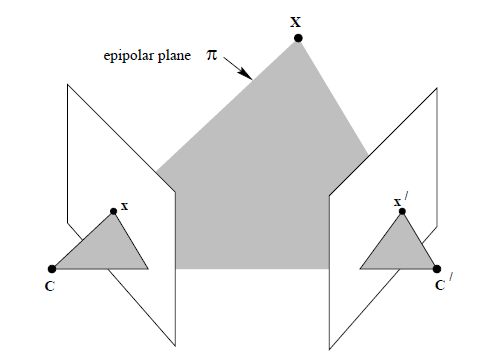
\includegraphics[scale=0.75]{Figures/Epipolargeomtrie.PNG}
    \caption{Epipolargeometrie}
\end{figure}
C und C’ sind hier die optischen Zentren der Kameras. Sie blicken auf einen Punkt X in der realen Welt. Die Ebene die durch die Punkte C, C’ und X aufgespannt wird nennt sich Epiolarebene. Die Punkte x und x’, die auf die Bildebene projiziert werden, liegen ebenfalls auf dieser Ebene. Die Schnittlinien zwischen der Epipolarebene sowie den Bildebenen sind die Epipolarlinien. Korrespondierene Punkte müssen auf den jeweiligen Epipolarlinien liegen. Da ein anderer Punkt X eine andere Epipolarebene aufspannen würde, wären dessen Epipolarlinien auch andere. Die Schnittpunkte der Basislinie (C – C’) mit der Bildebene sind die Epipole. Alle Epipolarlinien verlaufen durch die Epipole.

\subparagraph{Fundamentalmatrix}
Aus der Epipolargeometrie lässt sich die Fundamentalmatrix herleiten, die Informatio-nen über die extrinsischen Kameraparameter (Position, Orientierung) sowie die Intrin-sischen Parameter (Brennweite, Bildhauptpunkt) enthält. Sie stellt die algebraische Repräsentation der Epipolargeometrie dar. Die Fundamentalmatrix ist eine 3x3 Matrix und hat immer den Rang 2. Hat man einen korrespondierenden Punkt auf 2 Bildebenen x und x’, so muss mit der Fundamentalmatrix F gelten.
\\

$x'Fx = 0$
\\
Dies wird bei der Berechnung der Fundamentalmatrix noch wichtig. Sie wird über einen einen Datensatz an möglichen Punktkorrespondenzen über den 8-Punkte Algorithmus geschätzt.

\subparagraph{8-Punkte Algorithmus}
Der 8-Punkte Algorithmus ist der einfachste Algorithmus zum Schätzen der Fundamentalmatrix. Im speziellen wird hier der normalisierte 8-Punkte Algorithmus betrachtet, da die Normalisierung der Punkte zu besseren Ergebnissen führt.
Bei der Normalisierung werden die Punkte so verschoben, dass ihr Mittelpunkt der Nullpunkt ist, und zusätzlich so skaliert, dass deren Abstand im quadratischen Mittel sqrt(2) vom Nullpunkt entspricht. Die Normierung führt dazu dass das zu lösende Problem des 8-Punkte Algorithmus wesentlich besser konditioniert ist.
Der 8-Punkte Algorithmus basiert auf der Eigenschaft:
\\
$[x,y,1] F [x',y',1] = 0$
\\
Ausgeschrieben entspricht dies folgendem Gleichungssystem:
\\
$x'xf_{11} + x'yf_{12}  + x'f_{13} + y'xf_{21} + y'yf_{22} + y'f_{23} + xf_{31} + yf_{32} + f_{33} = 0$
Diese Gleichung kann nun umgestellt werden sodass
\\
$Af = 0$
\\
mit
\\
$A = [x'x, x'y, x', y'x, y'y, y', x,y,1]$
\\
und
\\
$f = [f11,f12,f13,f21,f22,f23,f31,f32,f33]^T$
\\
Die Fundamentalmatrix hat trotz ihrer 9 Einträge lediglich 7 Freiheitsgrade, da sie nur bis auf ihren Skalierungsfaktor definiert ist und die Bedingung an sie gestellt wird dass sie den Rang 2 aufweist. Daher kann mit mindestens 8 korrespondierenden Punkte-paaren über die Singulärwertzerlegung eine Lösung für f gefunden werden. Diese ist der Singulärvektor der zum kleinsten Singulärwert von A korrespondiert. Die Singulä-rwerte befinden sich in der Diagonalmatrix D. Zerlegt man A mittels Singulärwertzer-legung in UDV, so ist die Lösung in der letzten Spalte von V zu finden.
Für eine ideale Fundamentalmatrix müsste nach einer Singulärwertzerlegung gelten:
\\
$D_{ideal} = \begin{pmatrix} \sigma_1 & 0 & 0\\0 & \sigma_2 & 0 \\0 & 0 & 0 \end{pmatrix}$
\\
Dies wird in der Realität nicht vorkommen, da hier mit diskreten Pixeln gearbeitet wird und so nie die ideale Fundamentalmatrix berechnet werden kann.
\\
$D_{real} = \begin{pmatrix} \sigma_1 & 0 & 0\\0 & \sigma_2 & 0 \\0 & 0 & \sigma_3 \end{pmatrix}$
\\
Daher wird der dritte Diagonaleintrag von D auf 0 gesetzt und die Fundamentalmatrix aus den drei Matrizen aus der Zerlegung erneut berechnet.

\subparagraph{Schätzen der Fundamentalmatrix mittels RANSAC}
Um eine möglichst gute Fundamentalmatrix zu erhalten, wird der RANSAC Algorith-mus verwendet. Er nimmt sich aus der Menge der korrespondierenden Punktepaare 8 zufälllige Punkte heraus. Damit wird über den 8-Punkte Algorithmus eine Fundamen-talmatrix berechnet. Um die Güte dieser Fundamentalmatrix zu prüfen wird nun ermit-telt wie viele korrespondierende Punktepaare zu der berechneten Fundamentalmatrix passen. Dazu wird die Sampson Distanz ermittelt, welche sich wie folgt berechnet.
\\
\\
$d =  \dfrac{(x'^TFx)^2}{(Fx)^2_1 + (Fx)^2_2 + (Fx')^2_1) + (Fx')^2_2}$
\\
\\
$(Fx)^2_j)$ beschreibt hier den j-ten Eintrag im Vektor $(Fx)^2$.
\\
Liegt ein korrespondierendes Punktepaar unter einem gewissen Schwellwert, zählt er als Inlier und gilt als zum Modell passend. Diese Berechnung wird über viele Iteratio-nen mit immer zufällig ausgewählten Punkten für die Berechnung der Fundamental-matrix wiederholt. Die Fundamentalmatrix die die meisten Inlier hat, deren Modell also am besten zu den Daten passt wird jeweils gespeichert. Wurden alle Iterationen durchlaufen, wird die Fundamentalmatrix erneut über den 8-Punkte Algorithmus mit allen Inliern der besten Fundamentalmatrix berechnet.

\begin{figure}[ht]
    \centering
    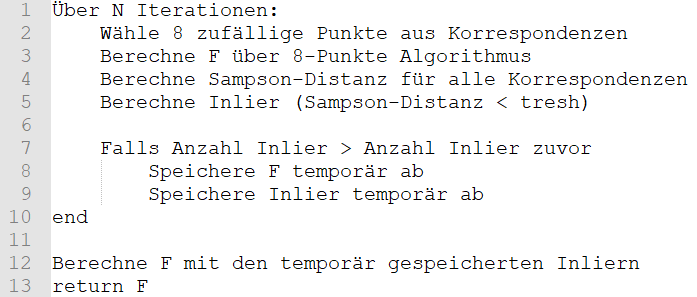
\includegraphics[scale=0.75]{Figures/PseudocodeRansac.PNG}
    \caption{Pseudocode RANSAC für Fundamentalmatrix}
\end{figure}

\subsection{Schätzen der Kamerapose aus der Fundamentalmatrix}
Um aus der Fundamentalmatrix die Kamerapose zu schätzen, muss diese zunächst in die Essenzielle Matrix umgewandelt werden. Diese steht in enger Verbindung zur Fundamentalmatrix, allerdings hat sie nur 5 Freiheitsgrade, nämlich 3 für die Rotation und 2 für die Translation (auch hier ohne Skalierungsfaktor). Um aus der Fundamentalmatrix die Essenzielle Matrix zu berechnen, muss diese mit der Intrinsischen Matrix des CameraParams Objekt, welches aus der Kalibrierung generiert wurde, multipliziert werden. Die Intrinsische Matrix enthält die Informationen über die Brennweite sowie den Bildhauptpunkt. Da hier alle Bilder mit der gleichen Kamera aufgenommen wurden, wird die Fundamentalmatrix zwei mal mit der gleichen intrinsischen Matrix multipliziert.
\\
$E = I' * F * I$
\\
Zunächst soll die essenzielle Matrix E in die schiefsymmetrische Matrix S und die Rotationsmatrix R zerlegt werden. Hierfür wird E mittels Singulärwertzerlegung in die Matrizen U,D und V zerlegt.
\\
$E = UDV$
\\
Zusätzlich werden die Matrizen W und Z benötigt:
\\
$W = \begin{pmatrix} 0 & -1 & 0 \\1 & 0 & 0\\0 & 0 & 1\end{pmatrix}$
\\
$Z = \begin{pmatrix} 0 & 1 & 0 \\-1 & 0 & 0\\0 & 0 & 0\end{pmatrix}$ 

Dabei ist W eine Rotationsmatrix und Z schiefsymmetrisch. Hier ergeben sich nun 2 mögliche Lösungen für die Rotationsmatrix:
\\
$R_1 = UW'V'$
\\
$R_2 = UWV'$
Beide Lösungen sind gültig und müssen später verifiziert werden. Der Transla-tionsvektor lässt sich einfach aus der dritten Spalte von U ablesen oder durch die Formel:
\\
$t = UZU'$
ermitteln. Aufgrund des fehlenden Skalierungsfaktors könnte die mögliche Lösung aber auch
\\
t = -t
\\
sein. Daher ergeben sich für die Kamerapose nun 4 mögliche Lösungen:
\\
$R_1, t$
\\
$R_1, -t$
\\
$R_2, t$
\\
$R_2, -t$
\\
Um zu prüfen welche Kameraposen die richtigen sind wird nun für jede Kombination eine Triangulierung der Inlier aus der Fundamentalmatrix Berechnung durchgeführt. Die erste Kamera befindet sich dabei im Nullpunkt mit der Orientierung eye(3), die zweite hat jeweils eine der vier möglichen Lösungen. Die genaue Vorgehensweise der Triangulation wird im nächsten Kapitel beschrieben. Bei der der Realität entsprechende Lösung, müssten (fast) alle in den 3D Raum triangulierten Punkte vor beiden Kameras liegen, bei den falschen Lösungen müssten sie hinter mindestens einer Kamera liegen. Zum Schluss werden die als richtig ermittelte Lösung noch in das Koordinatensystem der ersten Kamera überführt, indem die Rotationsmatrix transpo-niert wird und diese auf den Translationsvektor multipliziert wird. Dann werden sie als Pose der zweiten Kamera relativ zur ersten zurückgegeben.
\begin{figure}[ht]
    \centering
    \includegraphics[scale=0.6]{Figures/validierungDerLosungen.PNG}
    \caption{4 mögliche Lösungen}
\end{figure}

\subsection{Triangulation}
Die Triangulation ist eine Technik die aus Bildpunkten auf der Bildebene zweier Kameras Punkte im 3D Raum errechnet. Dafür wird eine Kameramatrix oder Projektionsmatrix benötigt. Sie ist eine 4x3 Matrix und enthält die interenen und externen Kameraparameter einer Kamera.  Sie beschreibt die Projektion eines Punktes in der realen Welt auf die Bildebene der Kamera.
\\
$ \begin{pmatrix} x\\y\\w \end{pmatrix} =  \begin{pmatrix} p_11 & p_12 & p_13 & p_14\\  p_21 & p_22 & p_23 & p_24 \\  p_31 & p_32 & p_33 & p_34  \end{pmatrix} \begin{pmatrix} X\\Y\\Z\\W \end{pmatrix}$
\\
Hier wird die Datenstruktur CameraMatrix von Matlab verwendet, die aus den Kame-raparametern sowie den zuvor berechneten Kameraposen die Kameramatrix errechnet.
Für die Triangulation wird die Form
\\
$x = PX$
\\
umgestellt in
\\
$AX = 0$
\\
A wird nach folgender Vorschrift aufgebaut:
\\
$A = \begin{pmatrix} xp^{3T} - p^{1T} \\ yp^{3T} - p^{2T} \\ x'p'^{3T} - p'^{1T} \\ y'p'^{3T} - p'^{T} \end{pmatrix}$
\\
Mit $p^i$ wird hier die i-te Zeile der Kameramatrix P bezeichnet. Die Punke x,y und x’,y’ die korrespondierenden Bildpunkte in Pixeln. Wird nur zwischen zwei Kameras trianguliert, so kann A genau wie in der Formel erstellt werden. Wird zwischen mehreren Kameras trianguliert, wie am Ende des Gesamtalgorithmus so kann A analog zu Abbildung X aufgebaut werden, mit jeweils 2 weiteren Zeilen für jede weitere Kamera.
Die Lösung für X wird über die homogene Methode ermittelt, indem A mittels Singulärwertzerlegung wieder in die 3 Matrizen U,D und V zerlegt wird. Die Lösung ist hier wieder korrespondierend zum kleinsten Singulärwert und daher, bei absteigender Größe der Singulärwerte in D,  in der letzten Spalte von V zu finden.
\\
$A = UDV$
\\
$X = V(end)$
\\

\clearpage

